\documentclass{article}

%IDIOMA
\usepackage[spanish]{babel}
\usepackage[latin1]{inputenc}  % Ambos para solucin de asuntos de idioma
\usepackage[T1]{fontenc}

%MATH
\usepackage{amsmath,amssymb,mathrsfs,mathptmx}  % Matemticas varias
\usepackage{hyperref} % Para escribir URLs
\usepackage{verbatim}

%IMAGES
\usepackage{graphicx}
\usepackage{epstopdf}
\usepackage{float}
\usepackage{subfigure}
\usepackage{wrapfig}
\usepackage[usenames,dvipsnames]{color}
\graphicspath{{./figure/}}
\DeclareGraphicsExtensions{.png,.jpg,.pdf,.mps,.gif,.bmp, .eps}
\usepackage{caption}

%VARIOS
\usepackage{multirow}
\usepackage{multicol}
\usepackage{tabulary}
\usepackage[table]{xcolor}
\usepackage{color}
\usepackage{listings}

\usepackage{tikz}


\begin{document}

\title{\Huge HPPS \\ \huge Informe 4 - Algoritmo de Dijkstra}

\author{ Juan Braun}
\maketitle

%\include{intro}
\section*{Introducci�n}
% v5.0: corregida por el tribunal.


El objetivo de este informe es comentar los resultados obtenidos para las diferentes versiones del algorimto de Dijkstra implementadas. 
El algoritmo de Dijkstra es un algoritmo de b�squeda en grafos. Dado un grafo $G = (E,V)$ donde $E$ son aristas con costos asociados y $V$ los v�rtices, el algoritmo calcula los caminos de menor costo desde un v�rtice inicial $s \in V$ hasta todos los dem�s v�rtices $v \in V-\lbrace s \rbrace$.   

A continuaci�n se muestra el pseudo-c�digo del algoritmo para el caso en que se usa la cola de prioridad. 
\begin{verbatim}

dist[s] = 0;  (distancia al vertice inicial)
for (todos los demas vertices)
   dist[v] = inf; (Las distancias a los nodos desconocidos es infinita)

S vacio; (En S voy guardando los nodos visitados)
build_heap(Q,V); (creo un min-heap Q con los vertices, se ordenan seg�n el costo)

while (Q no vacio)'   
   u = extractMin(Q) (saco el siguinte nodo con costo mas bajo)
   Agrego u a la lista de visitados S'      

      for (todos los vecinos de u)

         if dist[v]>dist[u]+costo(u,v) (si hay un nuevo camino de menor costo)
            d[v] = d[u]+costo(u,v) (actualizo costo)
            move_up(Q,v) (Reordeno el heap)            
         end if
      
      end for
      
return dist
\end{verbatim}

El caso en el que no se usa la cola de prioridad es muy similar, la diferencia esta en que cada vez que se quiere conseguir el siguiente de menor costo se oredena el arreglo con N recorridas.

El pseudo-c�digo que se muestra sirve para calcular los menores costos de un nodo inicial hac�a todos los dem�s, lo que se necesita en este caso es encontrar el camino de menor costo entre dos nodos dados. 

Para calcular el camino hacia un nodo en particular se necesita tener un arreglo en el que se almacenan los nodos previos con el costo m�nimo para llegar a ellos. Con este arreglo y sabiendo que cualquier tramo incluido en un camino de costo m�nimo es un camino de costo m�nimo para un nodo en particular, es posible calcular el camino m�nimo. 

Por ejemplo para el grafo de la Figura \ref{fig1}, cuando se busca el camino entre el v�rtice $A$ y el v�rtice $F$, se obtiene los siguientes arreglo con costos m�nimos y nodos previos. 

\begin{table}[h!]
\centering
\begin{tabular}{| l | c | c | c | c | c | c | c | c |}
\hline
V & A & B & C & D & E & F & G & Z\\ \hline
Costos & 0 & 25 & 20 & 25 & 25 & 20 & 10 & 30\\ \hline
Previo & nil & D & A & G & D & G & A & G \\ \hline

\end{tabular}
\caption{Costos y nodos previos}
\label{table:Prev}
\end{table}

A partir del Cuadro \ref{table:Prev} se puede calcular el menor camino de $A$ a $F$. Se mira el nodo previo de $F$, $G$. Ahora se mira el nodo previo de $G$, $A$. El camino de menor costo es $A \rightarrow G \rightarrow F$ 

\begin{figure}[h!] 
 \centering
    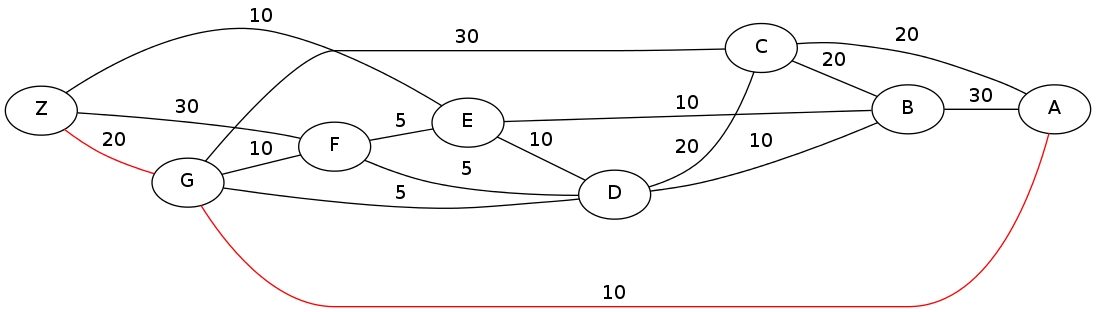
\includegraphics[width=1\textwidth]{Cami_dijkstra_1}
    \caption{Grafo de prueba}
    \label{fig1}
\end{figure}

La 


\section{Resultados}
Se midieron los ciclos de reloj para diferentes entradas. Los resultados obtenidos se muestran el Cuadro \ref{table:res}.

\begin{table}[h!]
\centering
\begin{tabular}{| l | c | c | c |}
\hline
 & \# nodos & \# ciclos con heap & \# ciclos sin heap\\[0.5ex]
\hline
E1 & 8 & 21 260 & 198 015\\ \hline
E2 & 50 & 154 892 & 2 917 770\\ \hline
E3 & 75 & 279 164 & 7 780 416\\ \hline
E4 & 100 & 538 346 & 17 863 372\\ \hline
E5 & 250 & 2 718 002 & 204 572 291\\ \hline
E6 & 500 & 9 950 835 & 1 442 783 202 \\ \hline
E7 & 750 & 21 601 507 & 4 652 164 219\\ \hline
E8 & 1000 & 37 042 054 & 10 718 859 780\\ \hline


\end{tabular}
\caption{Resultados}
\label{table:res}
\end{table}

\begin{table}[h!]
\centering
\begin{tabular}{| l | c | c | c |}
\hline
 & \# nodos & \# ciclos con heap & \# ciclos teoricos heap\\[0.5ex]
\hline
E1 & 8 & 21 260 & 31\\ \hline
E2 & 50 & 154 892 & 331.2\\ \hline
E3 & 75 & 279 164 & 541.16\\ \hline
E4 & 100 & 538 346 & 763.4\\ \hline
E5 & 250 & 2 718 002 & 2240.4\\ \hline
E6 & 500 & 9 950 835 & 4981.4 \\ \hline
E7 & 750 & 21 601 507 & 7912\\ \hline
E8 & 1000 & 37 042 054 & 10964\\ \hline


\end{tabular}
\caption{Resultados teo}
\label{table:res}
\end{table}

\begin{table}[h!]
\centering
\begin{tabular}{| l | c | c | c |}
\hline
  & \# relacion teorica & \# relacion obtenida\\[0.5ex]
\hline
E3/E2 & 1.64 & 1.81\\ \hline
E4/E3 & 1.4 & 1.92\\ \hline
E5/E4 & 2.94 & 5.04\\ \hline
E6/E5 & 2.22 & 3.66\\ \hline
E7/E6 & 1.59 & 2.17\\ \hline
E8/E7 & 1.39 & 1.71 \\ \hline


\end{tabular}
\caption{Comparaci�n resultados implementaci�n con heap }
\label{table:res}
\end{table}


\end{document}


